% !TEX encoding = utf8
% !TEX root = ../main.tex

% This content has been generated automatically from https://www.docx2latex.com/docx2latex_free and https://github.com/MartinoMensio/doc2latex_process_chapters 
% Consider editing the source Google Doc instead of this one!


\chapter{Approach}
\label{approach}

This chapter describes the design and the approach that has been investigated and developed to create a domain-specific bot. Section \ref{approachNLU} focuses on the major topic of this work, the Natural Language Understanding, treated as a really important component independent from the domain, by giving a description of the most relevant choices that have been done for the single-turn approach. These include word embeddings, that are really important to provide the proper meaning to words (from here the semantic denotation), and output dependency modeling, that enable to generate better output sequences for the slot tagging task. Then the novelty introduced for the multi-turn scenario is described to show the importance of the interaction context. The approach is defined as \textit{Deep Semantic Learning}, because the models are built from the observation of examples (\textit{Learning}) without manually selecting handcrafted features but relying on stacked recurrent layers (\textit{Deep}) that take as input the word embeddings that map words to a distributed representation that captures their meaning~\cite{sahlgren2008distributional} (\textit{Semantic}).

Then Section \ref{approachPrototype} describes the approach chosen for the selected applicative prototype, by starting from the target scenarios in \ref{approachScenarios}. A high level model is provided in \ref{approachModel} and then a personalization strategy is proposed in \ref{approachPersonalization} and the possible sources of information are described in \ref{approachIR}. The domain is the urban mobility: the bot goal is to provide a natural language interface towards the bike sharing service. Bike sharing is one of the projects for sustainable mobility that tries to address transportation replacement especially for the so called $``$last mile$"$ : cover more capillary with a public form of transport areas or trips that would be uncomfortable without using a private vehicle. With respect to car sharing, bikes have much little impact on the environment and are 100$\%$  \textit{green}. It is important to notice that not all the topics discussed in this chapter have been implemented. By comparing with the next chapter \ref{implementation} it can be seen that only the language understanding, the interface with the messenger platforms and the bike retrieval information have been brought to experimental environment.

%%%%%%%%%%%%%%%%%%%% Figure/Image No: 26 starts here %%%%%%%%%%%%%%%%%%%%

\begin{figure}[!htbp]
    \centering
    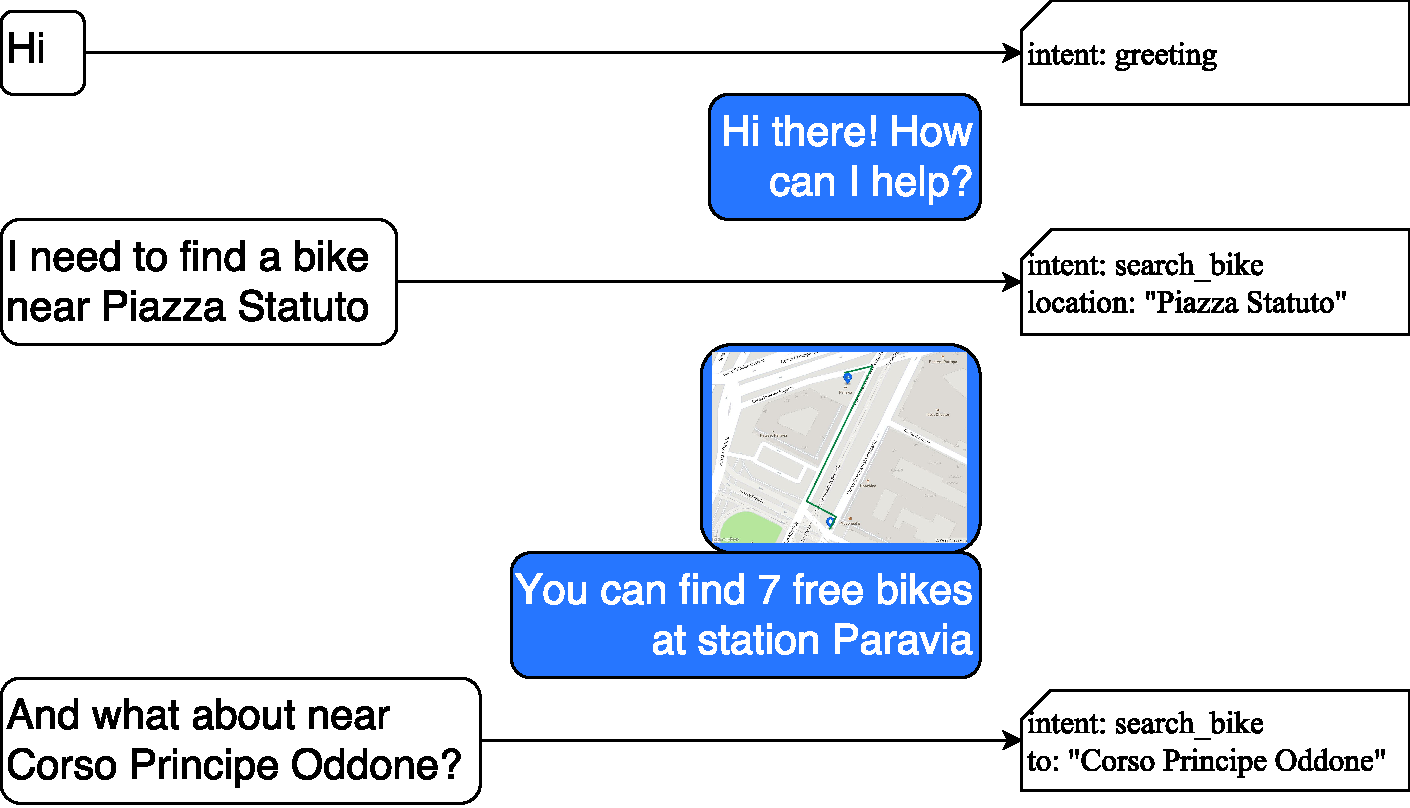
\includegraphics[max width=\linewidth,max height=8cm,keepaspectratio]{figures/multiTurnImportance}
    \caption{An example of interaction where the interaction context is important for the intent classification}\label{fig:multiTurnImportance}
\end{figure}

Figure~\ref{fig:multiTurnImportance} shows an example of interaction in the domain of bike sharing where the previous value of the intent is important to determine the intent of the last sentence, propagating over the dialogue.

\section{NLU}
\label{approachNLU}

Before describing the NLU module, it is important to remember the approach that has been chosen: it is NLU based, not generative. For this reason the dialogue management is still done using rules and the responses are provided by filling some templates.

Without having an existing corpus to train the dialogues in an end-to-end fashion, this is the approach that best fits the situation. For example some complex rules like $``$to search for a bike you should provide a search criterion or the last known position should be known and recent (2hr or ask for confirmation)$"$  is not manageable from a data-only focused approach. Inside this domain, it is better to provide static rules that are handwritten in some configuration files. Although there are several studies on end-to-end goal-oriented dialog, for the implementation of this prototype a rule-based logic has been chosen. The neural network are only applied in the NLU module that is responsible to extract intent and entities from the current dialog, eventually using the multi-turn environment only to better identify intents and slots.

\subsection{Single-turn NLU}
\label{approachSingleTurn}

The computational graph that has been chosen to perform the joint task of intent classification and slot filling is the encoder-decoder model proposed in~\cite{liu2016attention} because of its State of the Art condition. By simply providing the words contained in a sentence, both the intent and the slot tags can be computed. This approach was not modified for single-turn interactions, because the performance are already good as will be seen in chapter \ref{validation}. The focus has been on how to provide better inputs to the system in terms of word embeddings and on output dependency modeling for the slot filling.

\subsubsection{Word embeddings}
\label{approachWv}

The paper presenting the used model is not describing the way the words are fed into the network. The implementation provided by the authors\footnote{\url{https://github.com/HadoopIt/rnn-nlu}} however shows that a word embedding layer is part of the model and the values are randomly initialized. Since the datasets on which the evaluation has been done is not very big (especially the ones collected for the bike sharing domain), in the approach chosen fixed word embeddings, pretrained on bigger corpora, have been used as inputs. This actually gave a little boost on performances (see section [RE:validationResults]) on all the used datasets as can be seen in the evaluation section. Using pre-trained static word embeddings as inputs to the neural network can help reducing the number of tunable parameters and therefore help training small corpora, in addition to other advantages, like the ability to use word-similarity also with words that were not contained in the training corpus of the domain.

This is the most language-dependent part of the network and the goodness of the classification results highly depend on the quality of the embeddings.

Natural Language Processing techniques depend a lot on the selected language and also available libraries come with differentiated support based on it. Features such as Part of Speech, or Parse Trees, if they come from statistical models or handcrafted ones, can be good only if a lot of work is done in annotation of big corpora and therefore the efforts mainly fall on the English language.

Instead\ approaches\ that consider word embeddings are less dependent on annotated corpora, since those vectors can be built by simply having sentences in the desired language, that have been computed and realised publicly on the  Web, with unsupervised techniques. As mentioned before, the bot has as requirement to support also the Italian language. Concerning English,  several preprocessed word embeddings are available, trained with different corpora and with different algorithms. Concerning Italian, the found pre-trained embeddings are \textit{GloVe} and \textit{Word2Vec} trained by the Human Language Technologies of Pisa\footnote{\url{http://hlt.isti.cnr.it/wordembeddings/}} trained on Wikipedia and the official \textit{fastText}.\footnote{\url{https://github.com/facebookresearch/fastText/blob/master/pretrained-vectors.md}}\ A critical aspect to make word embeddings work at their best is to apply the same kind of tokenization both when training the word embeddings and when using them when feeding RNNs. For this application the choice has been to include punctuation in order not to discard any useful hints from the input sentences. An, hence, the two pretrained Italian embeddings have at their base a different tokenization method, removing punctuation and by applying other transformations (such as replacing hyphens and apostrophes with spaces to split the words),  the choice has been to recompute the GloVe vectors. This time the proper tokenization that, as will be seen in the implementation chapter at \ref{implementationWV}, has been applied to maximize the performance on a language that has a short representativeness in the domain-specific dataset.

\subsubsection{Output dependencies}
As mentioned in the state of the art section, modeling the output dependencies is very important in sequence labeling tasks. The different choices available are: feeding output labels as inputs to the decoding stage, or using a linear chain CRF. For its simplicity and also because it is mentioned in the referenced paper~\cite{liu2016attention}, the first one has been chosen.

In the description of the network in the paper it is not described how the output sequence labels are fed into the decoder. Different methods can be used: using one-hot encoding, that has the problem of scalability when the output dictionary is big enough, and word embeddings, to have a size independent from the number of existing slot labels.

%%%%%%%%%%%%%%%%%%%% Figure/Image No: 27 starts here %%%%%%%%%%%%%%%%%%%%

\begin{figure}[!htbp]
    \centering
    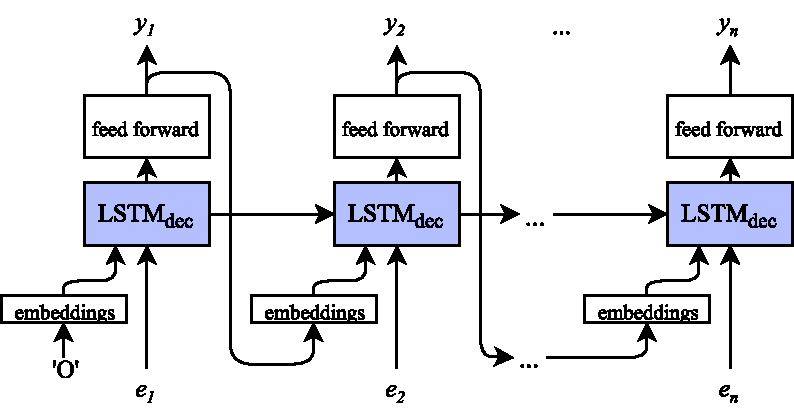
\includegraphics[max width=\linewidth,max height=8cm,keepaspectratio]{figures/outputDependencies}
    \caption{The selected approach to model the output dependencies}\label{fig:outputDependencies}
\end{figure}

The choice is to use word embeddings. This time however, differently from what happens to input words, the embeddings are on a separate dictionary: the IOB labels. For this reason they are not used pretrained but are included as trainable parameters of the computational graph. As can be seen in Figure~\ref{fig:outputDependencies}, the embeddings values are concatenated with the current encoded word coming from the encoder. The rest of the graph does not change.

\subsection{Multi-turn NLU}
\label{approachMultiTurn}

For solving the problem of multi-turn NLU, after analyzing solutions in the literature to the problem of keeping the context (like~\cite{xu2014contextual},~\cite{bhargava2013easy},~\cite{shi2015contextual},~\cite{serban2016building}), the decision has been to change the single-turn architecture to consider also previous sentences. The goal does not change: classify the intent and extract the slot values. So no advanced statistical dialogue-tracking techniques are used, but the change focuses to enrich the available inputs with contextual elements to do the selected tasks on the current sentence.

The work that follows for the contextual intent classification is taken from~\cite{mensio2018multi} done for the $``$Hybrid Question Answering with Structured and Unstructured Knowledge$"$  workshop,\footnote{\url{https://goasq.lri.fr/workshop/hqa18.html}} (in the following denoted with HQA2018).

Three main challenges are addressed:

\begin{itemize}
	\item detect the change of intent in a multi-turn environment: in other words, to understand dynamically when a certain session (sequence of messages related to a single intent) ends in favour of a new one. This corresponds to choose for each input sentence whether to keep the value of the previous intent or to consider some evidence on the current input. The first case happens when the input sentence is part of a preceding session, and the user is simply continuing the interaction with the same initial intent. The second case instead is when a new intent is expressed in the current sentence, signalling an intent change;

	\item capture intent dependencies using the RNN: capturing the sequences of intent values, a better prediction of the sentence can be done knowing the proceeding intents. This can be quite useful with sentences that are not so expressive because they are referring implicitly to some context of the interaction;

	\item consider the current agent turn words: having a knowledge about what has been replied to the user can help contextualize the new sentence that may not have evident indicators of the intent.
\end{itemize}

%%%%%%%%%%%%%%%%%%%% Figure/Image No: 28 starts here %%%%%%%%%%%%%%%%%%%%

\begin{figure}[!htbp]
    \centering
    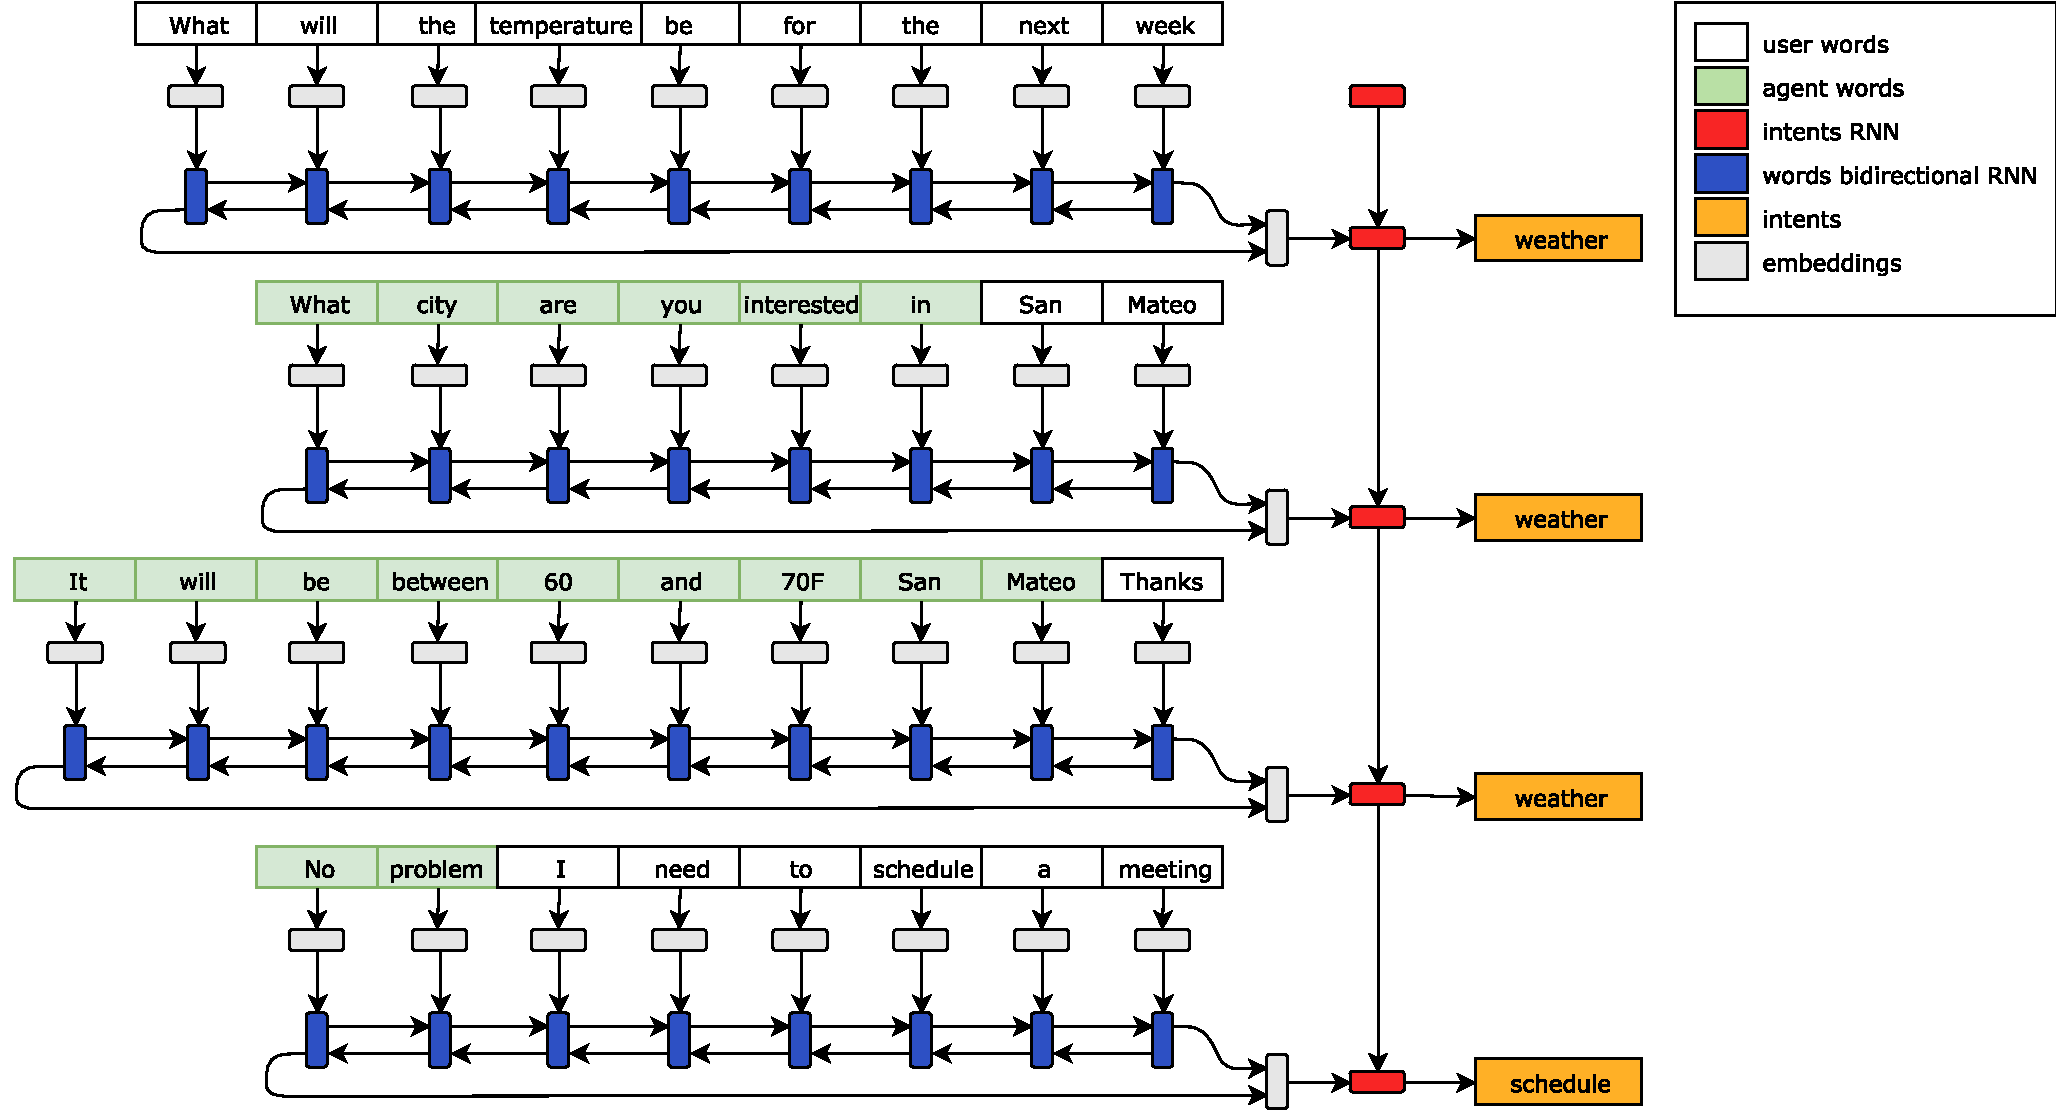
\includegraphics[max width=\linewidth,max height=8cm,keepaspectratio]{figures/approachMultiTurn}
    \caption{The selected Multi-turn approach}\label{fig:approachMultiTurn}
\end{figure}

Figure~\ref{fig:approachMultiTurn} illustrates our approach. Sentences are encoded in fixed-length vectors using the word-level bidirectional RNN (coloured in blue).The outputs of this first RNN are passed to a second RNN (coloured in red) that models the intent propagation of the user sentences over the different timesteps. This last RNN (in red) for each user sentence produces the contextualized intent value. The agent words are in green, while the words generated by the human are in white boxes.

In literature also other studies have been done on the problem of sentence classification inside an interaction context. The approach proposed in~\cite{xu2014contextual} on the classification of the domain, that is like the high level class in a hierarchical intent classification, uses the previous model prediction at word-level, concatenating it with each word vector.

The approach proposed in this work is different both in the specific point where the previous classification is used (not together with the input words but on the sentence level, using the high-level RNN) and also in the way the word-level features are summarized in sentence-level features and considered for next interactions by the learning network.

A critical point where this model should prove the goodness of the chosen cell, is when two completely unrelated sentence follow each others (e.g. two different intents). In this case the LSTMs/GRUs should learn to forget their past state in order to provide the new values. In inference time we can never know whether a certain sentence is a follow-up or is a new intent without any logical linking with the previous one, so the only good option is to train the network to learn when this happens. For this motivation, instead of training on single independent sessions, all the sessions have been concatenated. In this way the model will be able to work better both on sentences that belong to the same session (for example answering back to a missing slot) and on other independent questions (for example an independent intent).

\section{The bot for bike sharing}
\label{approachPrototype}

At the beginning of this chapter the domain-specific bot has been introduced as a Natural Language Interface towards the bike sharing information.

Since there is no agreement with the bike sharing providers (with the meaning that for the majority of cities supported the only way to obtain updated data is through web scraping, not through an official API), the information is only available in read mode, and only from public sources. For this reason the main things a user can do with the bot is to ask for information on the station and availability of bikes. No account linking is possible and users cannot unlock bikes using the bot. The main idea is to provide useful information to the users in a spatial context-aware setting. To provide this, the bot should analyze the area relative to the information and provide some suggestions to the user.

A required characteristic for the bot is to support the Italian language too: the agent, being developed in Turin, is supposed to be able to understand both Italian and English. For the sentences of the agent, the solution is simply to have both Italian and English template responses. Instead for the language understanding part, as will be seen especially for the Word Embeddings in \ref{approachWv}, it requires having the requested models for both the languages.

\subsection{Scenarios}
\label{approachScenarios}

We explain there the main scenarios that we want to face with this conversational agent. The main goal is to provide an easy-to-use interface that feels more natural for the user by allowing the interrogation in natural language.

\subsubsection{Search for bike stations information}
The main scenario is the one where a user asks for information about bikes and available parking slots. This can be expressed by a search of one station given some parameters or by a search that includes more stations.

For the first case, the user may want to find an available bike or a free parking slot given the current user position or another location. Instead for the second case, the user may want to ask for direction between two points: this involves finding a bike near the source and finding a place where to leave it near the destination.

The system, given simple queries expressed in natural language, should understand the request and extract the necessary parameters. The retrieval of information should include the interrogation of the bike sharing system or using cached versions, with the aim to find a path for the user that follows the constraints specified by the user and by the bike availability. Other sources of information that may be consulted are meteo information (to provide alerts for the given location) and routing information in order to return a path that can be used by bikes.

The history of conversation is stored in a way to find temporal and spatial pattern for the user, in order to build a model that can be used for personalizing his experience for example by providing places suggestions, as will be seen in \ref{approachPersonalization}.

If there is a place that can be suggested, with sufficient confidence of the recommending systems (telling that the suggestion is appropriate and relevant), additional information about it can be included in the response that is generated.

Such response should have the form of natural language, with the possibility to include visual contents such as pictures or links to more detailed information about the results.

\subsubsection{Search for supported cities}
Another scenario is when a user wants to understand the availability of the information for a specific city. In this case the request, expressed in natural language, will contain the name of the city. The system extracts it and finds if any bike sharing providers have support in it. If the city is not supported, information about which nearby locations are supported can be provided in the response.

\subsubsection{Small talk, refining the user model}
The last scenarios is the one of small talk: all the sentences that are not necessary to provide information about bikes, but are necessary to handle very basic chit-chat dialogues.

The user may use greetings, generic responses like yes/no, questions about the bot and other sentences that can be easily replied to, just to make it seem more natural.

Knowing that user expectations can be easily destroyed with a $``$\textit{I don't understand}$"$ , some answers have been added only to mitigate a very big problem that still is present and could only be solved with generative approaches.

Having some dialogues of this genre with the user could help understanding more about him, and this kind of information could be useful for refining the personalization model. By having a mixed-initiative interaction instead of letting the system to reply only to the questions, the bot may also ask questions to the user about his interests or explicitly asking for some feedback. In this way the personalization would receive a boost.

\subsubsection{Proactive messages}
Extending the mixed-initiative interaction out of the single dialogue, the bot may be able to actively begin the conversation with the user after some time of inactivity (not possible to start conversations with new users of course). This can be seen as breaking the idea of the bot as a service and for this reason should be only done if there is an advantage for the user. The advantage can exist in two different situations.

The first one is when, after having provided some kind of information to the user (e.g. a bike is available in a specific station) and before the user arrives there, the situation changes (e.g. the bike is no more available or the meteo is getting worse). In this case the bot could actively send a message to the user informing about the change.

The second situation is when a pattern in the behaviour has been observed (e.g. the user always searches for a bike at 8am in a fixed location). The system (some minutes before the forecasted event) can send an unsolicited message to the user informing him about the bike availability.

Those messages must be in some way controllable from the user. The suggested way of making them available is to test them once on the user and then getting the feedback: if the user reacts positively (measured by explicit response or interacting with the generated content) the feature can be kept on, otherwise the system will remember not to use the feature with the current user.

\subsection{High-level model}
\label{approachModel}

Given the main scenarios and given the fact that no publicly available corpus exists for the selected domain, the choice of the approach could not be in favour of an end-to-end system with dynamic response generation, but towards a NLU-based understanding. About the Information Retrieval, the data comes from external fixed set of APIs so it has been chosen to keep this approach instead of turning all the information in explorable graph of connected entities. These choices, together with the delineed scenarios, require the presence and cooperation of different components.

%%%%%%%%%%%%%%%%%%%% Figure/Image No: 29 starts here %%%%%%%%%%%%%%%%%%%%

\begin{figure}[!htbp]
    \centering
    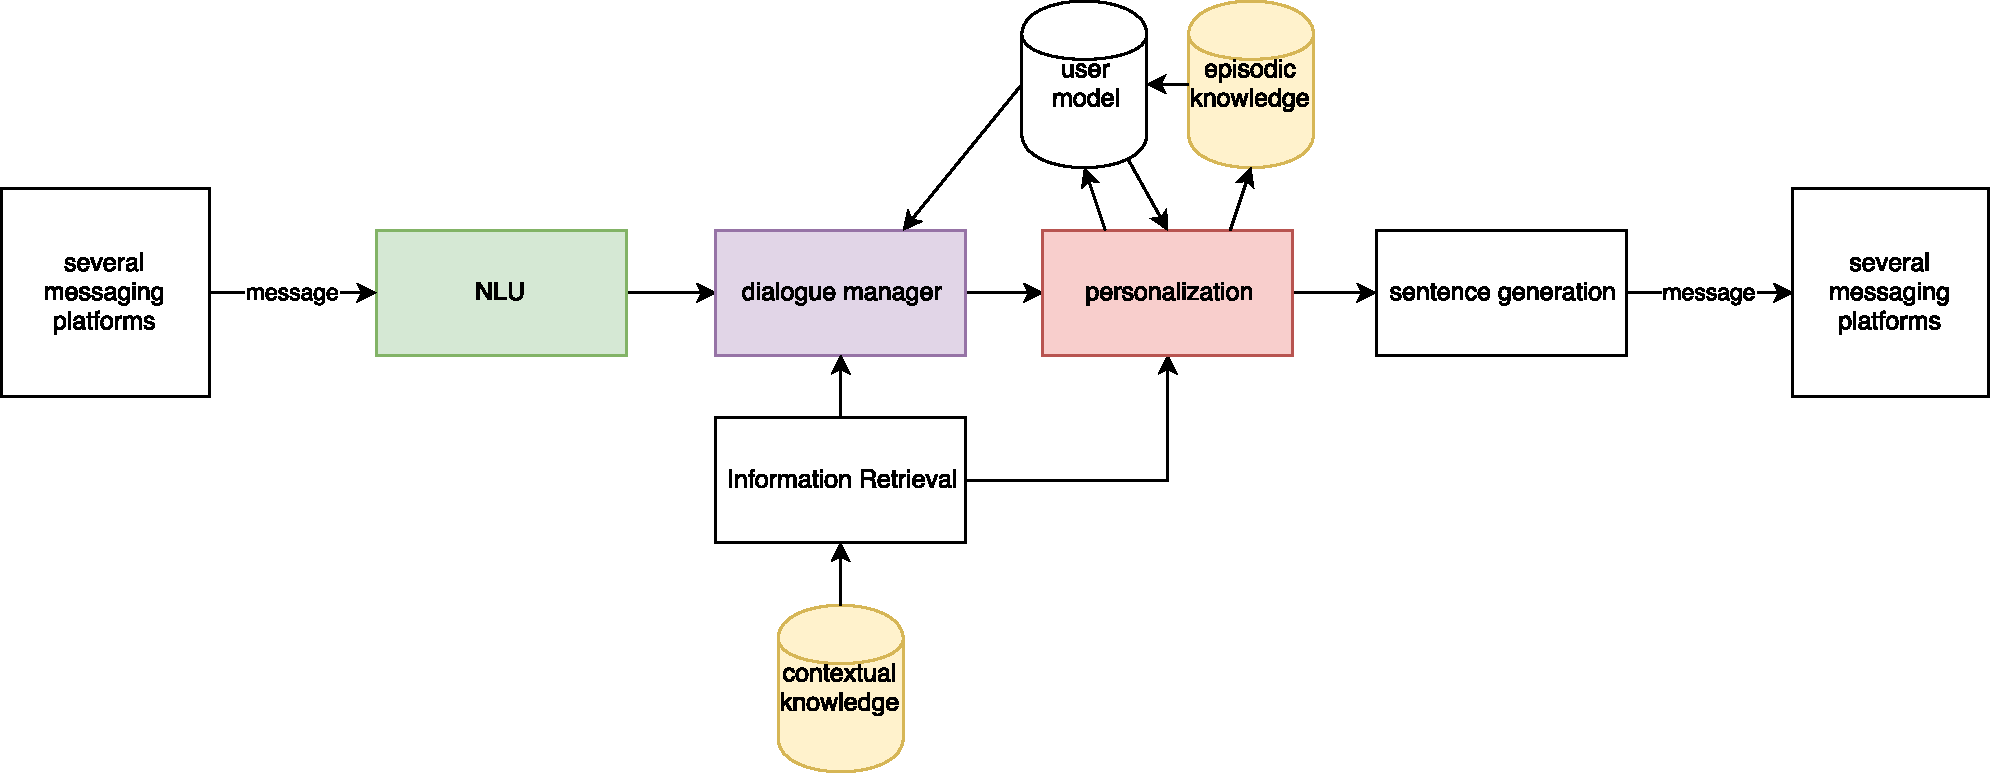
\includegraphics[max width=\linewidth,max height=8cm,keepaspectratio]{figures/systemHighLevel}
    \caption{The high level model of the system}\label{fig:systemHighLevel}
\end{figure}

As can be seen in Figure~\ref{fig:systemHighLevel}, one component is needed to interface with the different messaging platforms. This is responsible to make messages arrive to the $``$brain$"$  of the bot and to deliver responses back. Something about this component will be described soon and some implementation details will be given in \ref{implementationInteraction}. Then another component will do the NLU, providing intents and resolved entities. Passing through the dialogue manager, that contains the rules for managing the conversation, the flow will reach the personalization module that will collect episodic knowledge and together with the contextual knowledge will provide recommendations. The responses will be generated by combining the results and some templates will be filled.

The main sources of information (knowledge base) can be grouped together in two types: the Contextual and Episodic. In the first group can be found the providers of information, that are used in read only mode, inherent to bike sharing, places, meteo. The data is provided by external web API, and may be cached locally for performance improvements. The Information Retrieval module is responsible to manage them providing a higher level API that can be easily used by the dialogue manager. Instead the Episodic Knowledge contains records captured from the interaction with the users. Aggregated information can be computed and put in the user model that collects the user features that can be used for the personalization.

Going a bit deeper on the source and destination of messages, we are discussing about the messaging platforms where chatbot can be created. Nowadays there are so many different options available and every one of them has different features. There are even some of them that do not allow bot users. For example, the most widely used chat platform WhatsApp strictly forbids non-human accounts, punishing with permanent banning.

Starting with one of the first platform to support bots with official API, Telegram Messenger is surely the easiest platform to create bots on, allowing them since June 2015. Bot accounts can be easily created in few seconds with the only principle that the username should end with $``$bot$"$  in order to be recognizable. User can interact with bots using text, voice, buttons of different kinds, images (any kind of file can be sent) and including them also in chat groups. On mobile devices users can also send their location. This platform is the most friendly for bots, but is not widely used by non-geeks.

A very commonly used platform is Facebook Messenger, that opened to bots in April 2016. This platform is widely spread because is part of Facebook, and is available for every devices, also from web browsers. On Facebook Messengers the features are text/voice exchange, buttons of different kind, images and even attaching the user location. Facebook Bots have their Facebook Page and a few configuration steps need to be done to be able to set up a new bot. Other chat platforms that allow bots are Skype, Slack and Kik.

Other interesting communication channels are arising with expandible virtual assistants, that focus more on the use of the voice. Expandible in the sense that developers can develop some abilities for some domains and users are allowed to select them and add to the behaviour of the virtual assistant. We are talking about Alexa Skills and Cortana Skills. For these platforms the interaction with the user is quite different because instead of communicating directly with the user, the virtual assistant manages the conversation.

There are so many different platforms that it would be quite restricted to focus only on a single one. Furthermore the APIs change a lot between them, and even between different versions of the same platform.

Since all the details of the API are only an implementation detail, that will be fastly covered in the implementation chapter, here we will give only the motivation that lead the design of the system to be split into two parts: one will manage the channels and communication from and towards them, while the other will handle the important conversation stages (comprehension with NLU, dialogue state management, information retrieval, personalization). The message exchange between the two parts is done using a neutral representation, not dependent on any of the destination platforms.

This is what is intended with the term \textit{Multichannel Support}: the core of the chatbot can be put in communication with any messaging platforms, given that the message-proxy component (the part of the two that depends on the specific platform) is correctly configured. This component can make use of one of the many available solutions to manage different channels: Microsoft Bot Framework, Recast.AI Bot Connector, or start from scratch the implementation of the different endpoints. As will be seen in the implementation chapter \ref{implementationInteraction}, having this component has many practical advantages.

\subsubsection{Intent and slot types}
\label{approachTypes}

From an analysis of the scenarios, an hypothesis of the common user intents has been done, and from them also the slot types have been modeled. Intent and slot types have been successively refined in successive iterations by observing the transcript of some test users.

The results of some intents can be seen in Table~\ref{tab:nluTypes}.

%%%%%%%%%%%%%%%%%%%% Table No: 3 starts here %%%%%%%%%%%%%%%%%%%%

\begin{table}[H]
 			\centering
\begin{tabular}{p{0.79in}p{3.08in}p{1.79in}}
\hline
%row no:1
\multicolumn{1}{|p{0.79in}}{\textbf{Intent type}} & 
\multicolumn{1}{|p{3.08in}}{\textbf{Example}} & 
\multicolumn{1}{|p{1.79in}|}{\textbf{Slots}} \\
\hhline{---}
%row no:2
\multicolumn{1}{|p{0.79in}}{search\_bike} & 
\multicolumn{1}{|p{3.08in}}{Find me a bike near Central Park} & 
\multicolumn{1}{|p{1.79in}|}{LOCATION('Central Park')} \\
\hhline{---}
%row no:3
\multicolumn{1}{|p{0.79in}}{search\_slot} & 
\multicolumn{1}{|p{3.08in}}{Where can I leave the bike near Big Ben} & 
\multicolumn{1}{|p{1.79in}|}{LOCATION('Big Ben')} \\
\hhline{---}
%row no:4
\multicolumn{1}{|p{0.79in}}{plan\_trip} & 
\multicolumn{1}{|p{3.08in}}{I want to go from Piazza Castello to Porta Susa} & 
\multicolumn{1}{|p{1.79in}|}{FROM.LOCATION('Piazza Castello') TO.LOCATION('Porta Susa')} \\
\hhline{---}
%row no:5
\multicolumn{1}{|p{0.79in}}{city\_supported} & 
\multicolumn{1}{|p{3.08in}}{Is Torino supported?} & 
\multicolumn{1}{|p{1.79in}|}{LOCATION('Torino')} \\
\hhline{---}
%row no:6
\multicolumn{1}{|p{0.79in}}{set\_position} & 
\multicolumn{1}{|p{3.08in}}{I am in Rue de France, Nice} & 
\multicolumn{1}{|p{1.79in}|}{LOCATION('Rue de France, Nice')} \\
\hhline{---}
%row no:7
\multicolumn{1}{|p{0.79in}}{ask\_position} & 
\multicolumn{1}{|p{3.08in}}{Locate me} & 
\multicolumn{1}{|p{1.79in}|}{} \\
\hhline{---}
%row no:8
\multicolumn{1}{|p{0.79in}}{booking} & 
\multicolumn{1}{|p{3.08in}}{Please book me a bike near Piazza Navona} & 
\multicolumn{1}{|p{1.79in}|}{LOCATION('Piazza Navona')} \\
\hhline{---}
%row no:9
\multicolumn{1}{|p{0.79in}}{greeting} & 
\multicolumn{1}{|p{3.08in}}{Hi there!} & 
\multicolumn{1}{|p{1.79in}|}{} \\
\hhline{---}
%row no:10
\multicolumn{1}{|p{0.79in}}{info} & 
\multicolumn{1}{|p{3.08in}}{What can you do?} & 
\multicolumn{1}{|p{1.79in}|}{} \\
\hhline{---}
%row no:11
\multicolumn{1}{|p{0.79in}}{end\_discussion} & 
\multicolumn{1}{|p{3.08in}}{Ok} & 
\multicolumn{1}{|p{1.79in}|}{} \\
\hhline{---}
%row no:12
\multicolumn{1}{|p{0.79in}}{thank} & 
\multicolumn{1}{|p{3.08in}}{Thank you!} & 
\multicolumn{1}{|p{1.79in}|}{} \\
\hhline{---}

\end{tabular}
 \caption{Intent types and examples}\label{tab:nluTypes}
\end{table}
%%%%% TODO replace this table with next line
%% !TEX encoding = utf8
% !TEX root = ../main.tex

\begin{table}
  \begin{tabularx}{\textwidth}{lXX}
    \textbf{Intent type} & \textbf{Example} & \textbf{Slots} \\
    \toprule
    \texttt{search\_bike} & Find me a bike near Central Park & \texttt{LOCATION('Central Park')} \\
    \midrule
    \texttt{search\_slot} & Where can I leave the bike near Big Ben &\texttt{LOCATION('Big Ben')} \\
    \midrule
    \texttt{plan\_trip} & I want to go from Piazza Castello to Porta Susa & \texttt{FROM.LOCATION('Piazza Castello') TO.LOCATION('Porta Susa')} \\
    \midrule
    \texttt{city\_supported} & Is Torino supported? & \texttt{LOCATION('Torino')} \\
    \midrule
    \texttt{set\_position} & I am in Rue de France, Nice & \texttt{LOCATION('Rue de France, Nice')} \\
    \midrule
    \texttt{ask\_position} & Locate me & \\
    \midrule
    \texttt{booking} & Please book me a bike near Piazza Navona & \texttt{LOCATION('Piazza Navona')} \\
    \midrule
    \texttt{greeting} & Hi there! & \\
    \midrule
    \texttt{info} & What can you do? & \\
    \midrule
    \texttt{end\_discussion} & Ok & \\
    \midrule
    \texttt{thank} & Thank you! & \\
    \bottomrule
  \end{tabularx}
  \caption{Intent types and examples}\label{tab:nluTypes}
\end{table}

While the intents, once recognized, are ready to be used in a rule-based logic (each intent is linked to a set of actions that must be performed), for the slots more work needs to be done. First of all a check of the required ones based on the intent type, providing some questions back to the user to request them when missing. And then another component, the \textit{entity resolver}, needs to translate text spans into living entities. For the entities of type LOCATION this corresponds to translating a text into a location object with latitude, longitude, full name.

During the progress of this task many problems can arise. First of all, the user may refer to some place names that are bound to a position only for them: examples are $``$home$"$  $``$work$"$  and $``$school$"$  that are different for each user. For this reason this type of resolution and memorization is required to be personalized. Another common problem is the disambiguation of places with the same name that exists in different contexts. Geocoding can be biased on a specific area to give a preference on a certain bounding box,\footnote{ https://developers.google.com/maps/documentation/geocoding/intro$\#$ Viewports  } but the identification of this box is itself a problem because we can never know if the user is visiting some unusual places.

Apart of all those problems, the chosen solution is to use third party geocoding services to translate from a place name to a structured object that enables to work with the latitude and longitude to provide the desired path information. The problem of disambiguation and personalization are kept for future works.

The entity of type LOCATION can be inside the utterance as entity or can be the user position. Other entity types have not been considered for this initial prototype.

\subsubsection{Dialogue State Management}
The Dialogue State Management module is responsible to handle the mapping from intents and available slots to the actions and responses. For this part, as mentioned before, a rule-based approach has been chosen.

Each intent type is mapped to a specific set of actions. Additionally for each slot type that is used in a certain intent type a rule is configured to say if it is compulsory to have a value or not. In the case the slot is compulsory, the Dialogue State Manager must ask back for it, prompting a question to the user.

The intents that have been designed however have another type of rule: the location entity can be replaced by the current position of the user, that can be sent as attachment or expressed with the corresponding intent $``$\textit{set\_position}$"$ . If the value of the user position exists and is recent (last 2 hours), it can be used. Otherwise the user is required to provide it.

Once the requirements have been checked, the corresponding actions are called, involving the interrogation of the bike sharing information and other collateral sources. At the end, when the results are ready in a structured format, the translation back in natural language is done by filling some template responses with some item features.

\subsection{Personalization}
\label{approachPersonalization}

This section explains how the personalization techniques can be applied to the interactions with a chatbot, providing personalized content recommendations in a tailored communication fashion. This approach is composed of two main parts: \textit{content recommendation} and in this specific case the contents that are provided as recommendations are places around the user that he could be interested in. The second part is relative to the \textit{interaction itself}: the goal is to change the behaviour of the bot relatively to the mood of the user, in a dynamic way.

It is very important to notice that the topics here discussed have been used in a design phase but they have not been developed and tested. However we kept this section as part of this work because its content can be used for future studies (as discussed in Section \ref{conclusion}) that may implement the idea represented here. Furthermore, not only a personalization approach is presented, but also a bit of analysis of third party information providers that could enable this scenario, such as Facebook Graph API or Big Five predictors (in \ref{approachIR}).

\subsubsection{Content recommendation}
\label{approachRec}

For giving content recommendations, the objective of the recommender is to provide interesting places for the user around his trip. The area of search is therefore established by the results of the information: different strategies could be used to determine this surface, but the fastest one, that helps also querying providers of places information (e.g. Foursquare, Facebook Places, Google Places), is to use a circle determined by its center. As can be seen in Figure~\ref{fig:placesSearch}, the circle is centred in the mean point between the source and the destination, while its radius is chosen to cover the source and the destination plus an additional margin. The margin enables to provide also some places nearby the source or the destination that would be clipped out otherwise.

%%%%%%%%%%%%%%%%%%%% Figure/Image No: 30 starts here %%%%%%%%%%%%%%%%%%%%

\begin{figure}[!htbp]
    \centering
    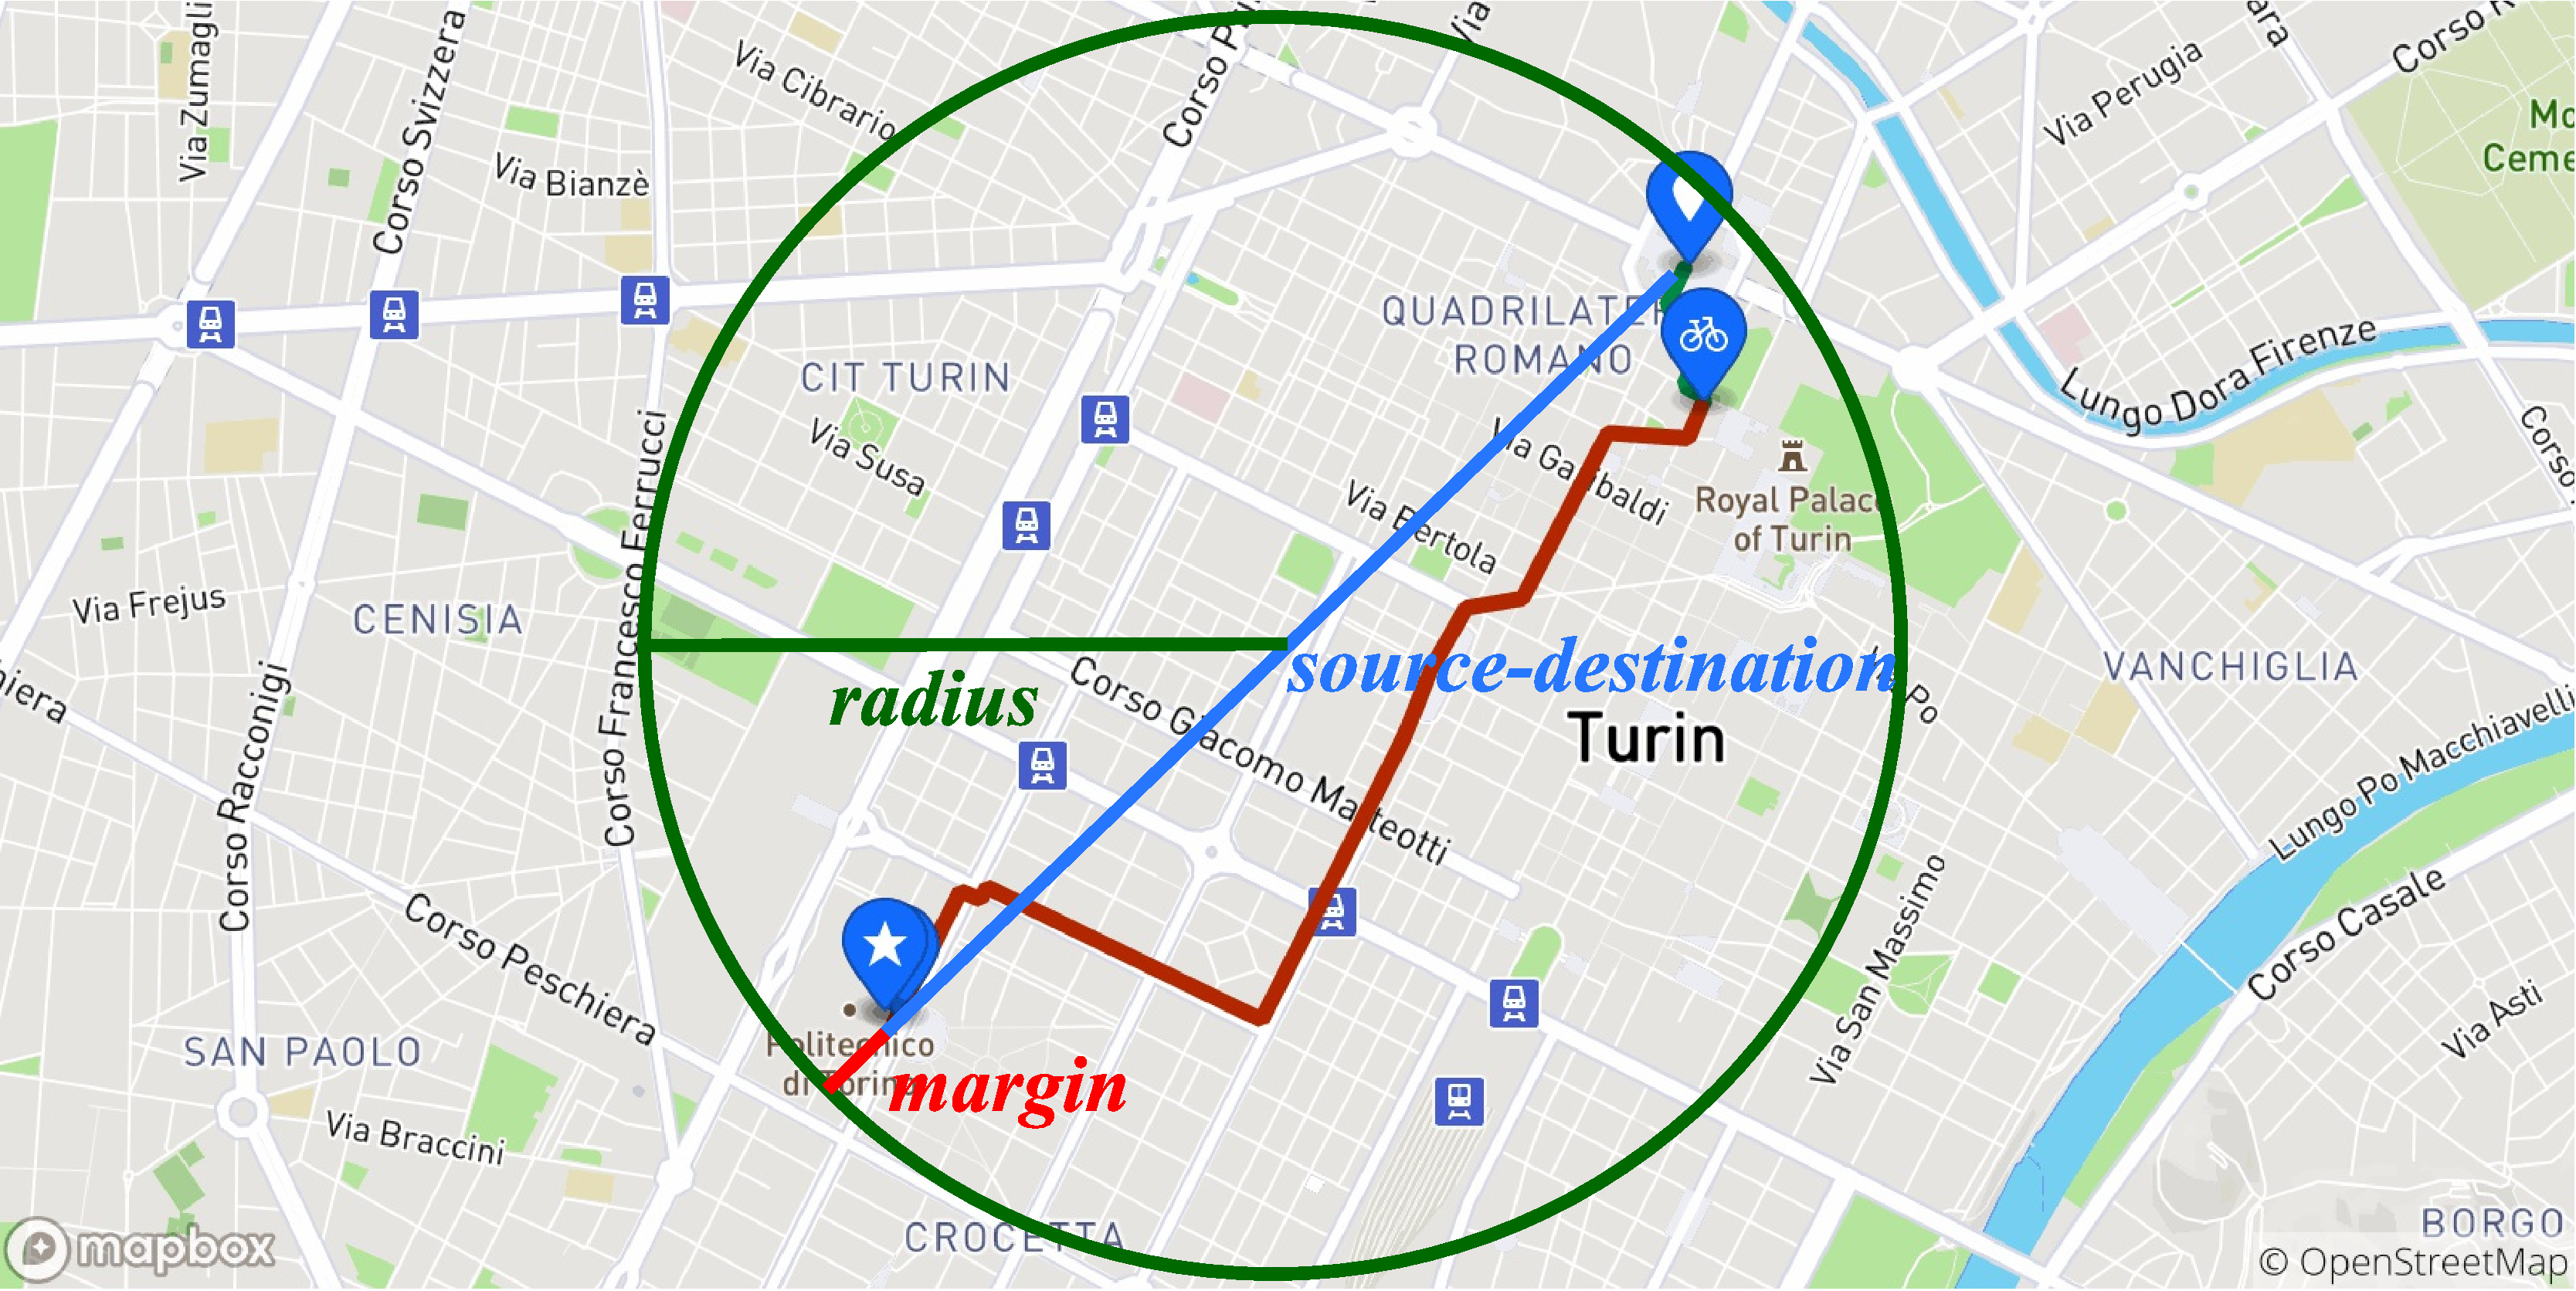
\includegraphics[max width=\linewidth,max height=8cm,keepaspectratio]{figures/placesSearch}
    \caption{The geographical constraints to search places for the recommendation}\label{fig:placesSearch}
\end{figure}

Determined the valid surface, the places in it are candidates for the recommendation. To restrict the places list and to provide one of them as recommendation, the strategy to be applied is to determine a place category that the user could be interested in. To find this category, a bit of user modeling needs to be done.

\paragraph{User modeling}
First of all, it is important to understand which variables need to be collected to build the user model. Some manifest variables like gender, age, profession, religion, political orientation are used for many profiling techniques, but not always they are available. Moreover, from a bot that is giving bike sharing information it is strange to be asked for those values, and can only make the user stop using the bot because it is asking strange questions. For these reasons, this kind of information is not even asked to the user.

As explicit data collection, some questions can be asked to the user in a more appropriate way, relatively to bike sharing. For example asking why the user makes use of bike sharing: to go to school, work or simply to run errands around the city. Having a general knowledge of the main purpose of using the bot should be really helpful, extracting personal details like occupation or student status. This type of information can be collected at the beginning as bootstrap questions, or also after some dialogue with the user has been done. In this way the user can soon use the service without being blocked by bootstrap questions, but after some minutes of inactivity he can be sent some questions in order to improve the service. In any case, waiting for responses should not block in any way the understanding process of new requests. For this reason it is important that the classification of intents continues to work, distinguishing dynamically if the user is keeping the discourse in the bootstrap environment or if he is providing his own intent to reach some details about bike sharing. 

Other explicit information can be collected when the recommendation is in act, as feedback to the suggestions: feedback can be positive or negative, collected through specific buttons or intercepting the user clicking on the information given about the place. The feedback can help refining the user interest and also understanding his attitude towards recommendations (as will be seen in subsection \ref{approachPersonalizationCommunication}).

As implicit user modeling, observing the patterns (temporal and spatial) of the queries performed can help find users similarity and improve the collaborative filtering approach (as will be described soon). The patterns in the spatial dimension correspond to frequent places, while in the temporal dimension can be interpreted as habits.

Other optional sources of data may come from social networks. On social networks people usually show their interests towards different kind of things: check-ins, places, music, films, and many others. This can be very helpful to user modeling, both providing user features both providing item (places in this case) features. The inputs in this case are the interests of the user, that can be provided by doing a login on the desired social network. The access scopes\footnote{\url{https://developers.facebook.com/docs/facebook-login/permissions/}} usually can be requested with different granularity levels and allowing different types of personal information to be retrieved. This login is proposed to the user as optional and if denied must not preclude any functionalities of the bot. Simply the model for this user will not be accurate and more generic recommendation will be provided.

Given the social network footprints, a prediction of the \textit{big five} personality traits can be done using some online available APIs (see the related Information Retrieval description in \ref{approachIRbig5}): the user features will be the \textit{big five} together with \textit{concentration} on different areas (like art, biology, business, IT, education, engineering, journalism, finance, history, law, nursing and psychology). These features try to describe the personality and the possible interests of a person, and can be computed easily as will be seen in the section. Furthermore, as described previously in \ref{soaPersonalizationFeatures}, they come from expert psychological studies~\cite{costa2008revised} and are proved to be able to predict unpublished user features~\cite{kosinski2013private}.

Once these user features are collected, different recommendation paths have been modeled to suggest the categories of places inside the selected area.

\paragraph{The trainable relationship}
The recommendations of categories are given following an hybrid recommendation approach, combining content-based with collaborative techniques. As can be seen in Figure~\ref{fig:recommendationPaths}, there are different entities involved, but the main goal is to learn the mapping from user features to place categories. This is the unknown relationship evidenced in red in the figure. The model needs to retrieve as many details on the two edges of this relation, in order to be more able to suggest the best places for each user.

%%%%%%%%%%%%%%%%%%%% Figure/Image No: 31 starts here %%%%%%%%%%%%%%%%%%%%

\begin{figure}[!htbp]
    \centering
    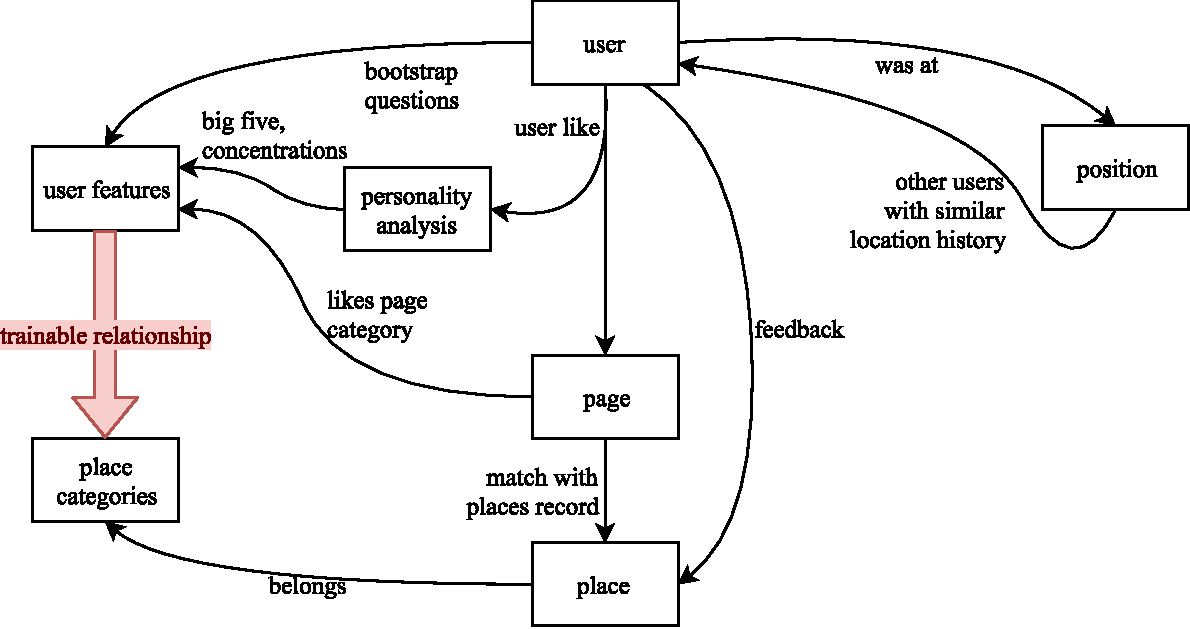
\includegraphics[max width=\linewidth,max height=8cm,keepaspectratio]{figures/recommendationPaths}
    \caption{An overview of the possible recommendation paths between the user and the places}\label{fig:recommendationPaths}
\end{figure}

There are different ways to collect the details of user or of the places. The user features they have just been described, but to have a correlation between them and the places features, it is necessary to collect also information on the other side of this trainable relationship. For this reason, when connecting to third party social networks (gold candidate is Facebook), the desired scopes for this personalization strategy should allow exploring the user interests (Facebook \textit{Likes}) and the places where the user checked-in (similar to the Foursquare checkins, Facebook calls them as \textit{user tagged places}). The first ones, besides allowing to infer user features, allow exploring the places he likes, because pages can have a physical location. The places that have been visited or have been $``$liked$"$  by the user can be used to analyze the respective categories, and add training data.

Yet another input can be used to feed data about this trainable relationship: explicit and implicit feedback. Receiving signals from the user about a recommendation, the model can be refined depending on the positivity of the user opinion. The explicit feedback is acquired when the user evaluates the solution, and the implicit can be collected by using a link rewriting strategy that captures when a suggestion link is visited.

All those inputs are used to train this relationship that models how different users with similar interests are likely to appreciate places with similar features. To model this unknown mapping, a simple feedforward neural network can be used and trained with the data of every user. It is a content-based component because users that have expressed a positive opinion on a certain category, will receive recommendations with places that have similar characteristics. But it is also collaborative because the relation is trained with data of all the users, so similar user features map to similar places features.

\paragraph{Providing recommendations}
So given any user and any constraining circle around his path, different recommendation strategies can be applied depending on which inputs are available.

First of all, the trained relationship can be exploited if enough inputs are known. This is the case where the user has done the social login and/or has provided answers to the bootstrap questions. Using his feature vector, an estimation of the categories he is interested can be done by applying this hybrid recommendation component. Once the categories are found, the search within the bounding circle can be performed by giving preference to them.

If the user feature vector is not yet populated, or the previous recommendation strategy gives results that have low confidence, another strategy is to use the explicit feedback provided on previous recommendation. This time, no hybrid recommendation is used, but only a content based one, suggesting places with a similar category to the ones that were previously appreciated.

If also this kind of information is not available, but the user has used the bot for a while receiving several times path directions, another strategy can be applied. The idea is that users with similar spatio-temporal usage patterns are somewhat similar, because they go to the same places around the same time. Following this idea, an analysis of those patterns can be done by applying some unsupervised techniques, such as user clustering based on the Episodic Knowledge. The features to include for this clustering are time and space of the locations involved while performing the interaction with the bot. As output from this application of clustering we can get a neighborhood of the user in this space of spatial and temporal features. We can then use the identified similar profiles and ask the recommender a suggestion with respect to them, and see the effect of propagating this recommendation to the starting user. This technique is therefore really collaborative.

However all those strategies rely or on a properly featured user (to use his feature vector), or on a wide usage by different user (to enable the neighborhooding search). Those aspects are heavily suffering from the cold start problem. To mitigate this effect, especially on the first epochs of the system where a very limited number of users are interacting with it, a last technique can be used. Places API, as will be seen in the section relative to the Information Retrieval \ref{approachIR}, usually provide a section named $``$trending places$"$  (in the jargon of Foursquare they are called \textit{top picks}). This kind of places usually represent very interesting places in general, that can be safely suggested to the new users. An important role again is played by collecting the feedback after prompting the suggestions. Generic recommendations can be given at the beginning and can be slowly refined by collecting the feedbacks and collecting more users that hopefully will accept to perform the social login.

When a certain distribution of probability over the place category is computed, there are still some choices that can be performed to reinforce the recommender system. One of them, typical of the reinforcement learning, is the \textit{exploration vs exploitation dilemma} that in this case can be seen as: it is better to provide an experimental suggestion that has a low confidence score and could result both in a serendipitous acceptance and brutal rejection, or to provide a more confident suggestion that can be seen as foregone and will not help discovering more about the user? 

To put this dilemma into action, an $ \varepsilon $ -greedy~\cite{tokic2010adaptive} can be used to dynamically determine a \textit{temperature level~\cite{hinton2015distilling}} that will model the softmax smoothing. A low temperature value makes the recommendation more confident and stays on the exploitation side, while an higher value tends to make the choice over the categories more random, on the explorative side.

If this approach is implemented, measures of its goodness should consider not only the accuracy of recommendations, but also their diversity and serendipity.

\subsubsection{Tailored communication}
\label{approachPersonalizationCommunication}

How introduced previously, we think that the personalization strategy in a textual environment should not be limited to content recommendation. Being human conversation itself one of the most dynamic interactions where it is very important to understand the interlocutor to say the things in the right way, in the following paragraphs different modifications to the mean itself of interaction are considered. First of all, some operative modes are defined to represent different behaviours with respect to the recommendation process. Then a memory of the personal preferences, letting the bot remember things that can be useful to fasten the interaction (having places saved with names like $``$home$"$  and $``$work$"$ ). And finally some considerations that can help reducing the linguistic style distance between the user and the bot.

\paragraph{Operative Modes}
Starting from the operative modes, we can define them as states of conversation that model how much the recommendation process should be active and visible to the user. It should reflect how much the user is willing to receive suggestions relatively to interesting places in addition to the normal information about the trip.

Three operative modes can be designed:

\begin{itemize}
	\item Normal: the recommendation are provided when the system is sufficiently confident. This means that not for each search a recommendation is provided, because that would be too much, but sporadically a place is suggested and the effect on the user is observed;

	\item Straight to the point: the user expressed negative sentiment in response to a recommendation, or may be in a hurry and needs only the bike information. In this situation, the bot is not allowed to send recommendations because can lead to a very negative attitude and abandonment of the conversation;

	\item Conversational: the user is chatting with the bot, asking some questions about it. This may be the right moment to ask some information to the user in order to refine the model. Questions should not be too personal, but always somewhat related to the topics discussed. An analysis of the personal interests can be done to understand better which categories can be interesting for him.
\end{itemize}

For deciding which operative mode should be applied, it is very important to collect signs from the users. Signs can be explicit in feedbacks: both textual or by using some buttons next to the results. Signs can also be implicitly sent in text messages: latent sentiment analysis can sometimes provide sporadic hints.

Or signs can be collected from monitoring the destination pages that are linked in the results. For this reason the strategy of link rewriting can be used to intercept the user clicking on the details of the recommendation: an intermediate webserver can be set as the destination when creating the link; when it receives the request, it records the fact that the user has reached it and sends a redirect for the real destination. This strategy is widely used to measure click-through rates by all the big companies (see for example the real URL used in the results of a Google Search, or the links built by Facebook and Twitter).

\paragraph{Personal preferences}
The personalization, beyond providing the recommended content in the correct way, should also consider some personal preferences that may enable a faster and more comfortable usage, like setting bookmarks or saving form fields in a web browser. In the domain of bike sharing, it can be useful to let the user save favourite stations, linking them with a shorter name, or saving the values for other commonly frequented places, like the home or the work/study location. By having this personal map between names and locations, searches can be performed faster and without the need to remember long addresses every time.

Other preferences that can be saved for the bot, are values that play the role of settings: set automatic messages in certain time slots, to receive unsolicited messages for bike availability on recurrent habits or to receive constant updates about a bike station in the minutes before its usage. Those are all things that could enhance the user experience.

\paragraph{Linguistic style and mood}
Furthermore, the personalization strategy could also be expanded to the linguistic style of the user. This can declinate on a targeted choice of language or the usage of emotions. Those enhancements can be used effectively only if responses are provided in a generative fashion.

On the choice of language, what can be done is a imitation of the formality level and jargon. This is what happens in real life dialogues, where the terms people choose are usually targeted to the interlocutors and the sentences are generated to fit the social situation. In a generative approach, as works like~\cite{li2016persona} show, the language can be modified by being more user centric with respect to speaking style, that can reflect also some background information of the interlocutor.

Instead on the side of emotions, as~\cite{zhou2017emotional} shows, the output of generative approaches can be biased on a specific emotion. This can help making the user more understood by reflecting his mood of writing. However, as discussed in the introduction, this emotional content has many potential negative effects on the personality and should be evaluated well in ethical field before giving any implementation.

\subsection{Information Retrieval}
\label{approachIR}

This section analyzes the kinds of information that both have been used in the prototype and may be used for the implementation of the personalization approach. Some details are given about each data source that is necessary, together with the respective APIs that can be used. The sources of data cover different domains: from the bike sharing information, passing through the computation of directions and geocoding, and going in the direction of personalization by means of APIs to retrieve the recommendation items or APIs to compute user features. Below are listed the different data sources that need to be queried to provide updated information to the users.

\subsubsection{Bikes}
Bike sharing is an expanding market, where every day more companies are investing in and more people decide to use them for their relatively small cost and for their easiness in the urban environment. The majority of the providers have station-based systems, where the users begin and end their trip at fixed locations (the stations). However nowadays station-free systems are being spread in major cities, with the advantage of being able to leave the vehicle in any responsible place.

Given the multitude of companies and the economic competition between them, and also the fact that in different cities multiple providers are available (e.g. in Turin there is the station-based toBike and the station-free oBike and MoBike), interfacing with them is quite difficult for two reasons:

\begin{itemize}
	\item The bike sharing providers may not want to make available their data to third-party players, both for privacy issues (data disclosure can be quite a problem also in this domain\footnote{\  Zoey Chong. (2017, December 6). Obike becomes latest victim of global data breach. CNET. Retrieved from https://www.cnet.com }) and because of its value;

	\item The data format is different for each bike sharing system.
\end{itemize}

For these reasons, the only applicable approach to get the desired information is to use some open-source contributive library that is produced and maintained by a sufficient number of people in order to cover a big number of cities. The information may be extracted by publicly-available APIs or by web scraping techniques.

Fortunately such library exists for station-based systems: pybikes.\footnote{\url{https://github.com/eskerda/pybikes}} This library interfaces with different bike sharing providers by using open RESTful APIs when available or using web scraping to connect to other ones. The structured information about the bikes and stations can be updated from the source and be used for any computation. Being completely open-source, everyone can contribute and make it work for additional systems.

\subsubsection{Geographical information}
Instead on the side of geographical tools, two main needs are addressed: geocoding capabilities, as tools for the entity resolver that needs to turn textual entities into geographical objects, and the computation of paths between sets of points with specific constraints.

For the geocoding capabilities, translating text into positions can be achieved by using online services such as Google Geocoding Service,\footnote{\url{https://developers.google.com/maps/documentation/geocoding/intro}} OpenStreetMap Nominatim,\footnote{\url{https://nominatim.openstreetmap.org/}} Mapbox\footnote{\url{https://www.mapbox.com/geocoding/}} or many others. Among them, Google seems to be the most reliable and comprehensive even in terms of incomplete textual descriptions. The query can ask even for preference in a given bounding box, and the response provides back a list of candidates. The information retrieved through this service provides the source and destination points used to search the bike stations and to compute the paths.

Given the locations of source, destination and possible stations involved, a path has to be computed to give directions to the user with the selected constraints. Since many web APIs exist with good results, the approach is to find a service with the desired functionalities and use it. The main feature requested is to compute paths that are suitable for cycling: respecting the street laws, avoiding highways, preferring cycle lanes are just the examples that show how important the mean of transport is while computing the paths. Looking for this functionality, three major providers have been analyzed. First of all, the Google Maps Directions API,\footnote{\url{https://developers.google.com/maps/documentation/directions/}} that should support bicycle directions. But however the service does not work in the city of Turin, so it has been discarded. The second system considered has been one of the many based on the OpenStreetMaps information: OpenCycleMap.\footnote{\url{https://www.opencyclemap.org/}} Even though the information provided should be the most accurate because of the collaborative open source data, it seemed too much complicated to integrate and had some strange behaviour that made it not totally reliable. The last and definitive service has been the Mapbox Directions API,\footnote{ https://www.mapbox.com/api-documentation/$\#$ directions  } fully supporting bike paths and having only as negative point a limited number of calls per month (50000 that is quite huge though).

A feature that would have been interesting to consider is the possibility to choose the path with criterions different from shortest or faster, for example considering the smells and happiness of the places in the route. This could potentially provide results that offer a better quality of the path, but have currently be done as an experiment only in the city of London~\cite{quercia2015smelly}~\cite{quercia2016emotional}~\cite{aiello2016chatty}. This feature was not considered, in favour of the usual optimal path.

\subsubsection{Places}
Instead for the information about the places, required for the recommendation strategy described above, there are different options that can be considered.

The first one is again by Google with the Places API,\footnote{\url{https://developers.google.com/places/web-service/search}} that provides up to 1000 requests per day freely. A similar role is played by Foursquare that makes available different tools for place discovery: one traditional place search API\footnote{\url{https://developer.foursquare.com/docs/api/venues/search}} that can be used to search places by name, location, category or other criterion and can be used also to match places from other external sources (like the pages that some user expressed interest to, that can be used with the $``$match$"$  intent that requires the position to be the same with high precision); an explore API\footnote{\url{https://developer.foursquare.com/docs/venues/explore}} that can be used to search for relevant places inside a selected area on a given section (that corresponds to high level categories: food, drinks, coffee, shops, arts, outdoors, sights, trending, venues frequently visited after a given one, or a mix of recommendations generated without a query from the user called topPicks). This second API can be used to get more recommendation-related items against search-related results: the objective of search is really different. Furthermore the call limits of Foursquare are even bigger (120.000 requests per day) and this makes it the best candidate for the required features.

\subsubsection{Facebook Graph API}
The personalization approach described before requires an analysis of social networks to perform an analysis of user features and the pages and places that are liked by them. Nowadays the most widespread social network is undoubtedly Facebook. With around 1.4 billion users active daily,\footnote{\url{https://zephoria.com/top-15-valuable-facebook-statistics/}} it is a mine of data that gets fed constantly with multimedia content. Users tend to voluntarily disclose personal details on this platform, following the pages of the places they have been to, self-tagging themselves in places to show their experiences to their friends, personal interests like music, films and arts. This is the perfect source of profiling that can be found. For this reason, a quite cumbersome management of read permission has been developed in order to make users a bit more conscious about what they are sharing with applications linked to the platform.

For example chatbots, when messaged by users, only see their name, picture, locale and gender. To see other details a Facebook Login\footnote{\url{https://developers.facebook.com/docs/facebook-login/permissions/}} needs to be performed. This login can be done on any messenger platform because the procedure is handled by a flow that only requires to have a web browser installed that will carry some authorization information towards a destination web server that is configured as endpoint.

The login follows this flow. First of all, the bot provides an url to login on facebook, specifying the destination endpoint URL (owned by the developer and configured on the corresponding Facebook Application as trusted domain). Then the Facebook login is shown to the user, that authenticates himself and selects which permissions to give to the application. After this, the user is redirected to the endpoint URL with a parameter that contains a short-term token usable to retrieve the user information using the Graph API.

The identified scopes that are necessary to retrieve both the user likes and the tagged locations are $``$user\_likes$"$  and $``$user\_tagged\_places$"$ . The data obtained can be used to estimate the personality traits and to obtain a list of place categories that the user has shown interest for. To make the correspondence between Facebook places and Foursquare places, the intent of matching is specified to the places search API.

\subsubsection{Big Five computation}
\label{approachIRbig5}

Another third-party component, that is very useful for the personalization approach, is the computation of the \textit{big five} personality traits~\cite{goldberg1993structure}. Since having a mapping from personal preferences and tastes to this five-factors representation requires a lot of training data, it is quite infeasible to start from scratch without an existing dataset. For this reason, a search of online services has been done. The requirement that we searched for, beyond free usage, is to avoid personal detail disclosure. For this reason only solutions that allow anonymous data to be sent and retrieved were considered (no third party application login, only sending anonymous features to obtain a response over the personality traits). In an exploration phase, an interesting service has been found, that only requires a list of facebook pages identifier to compute the personality traits. This service is ApplyMagicSauce,\footnote{\url{https://applymagicsauce.com/research.html}} that can be used both on their site, allowing their application to read the personal profile, or can be used as a web service, sending simply the list of pages in any way indicating which user is linked. The results provided are both the big five and some concentration areas described before. They can be used to fill the user vector and to understand better his personality.

\subsubsection{Other}
Other additional data sources can refer for example to the weather conditions. Being bikes vehicles subject to bad weather conditions, considering precipitations could be advantageous for the user. For example while retrieving the information for a trip, the bot could warn the user of an imminent storm.

Different weather API are available online, and the criteria to choose which one to use should be the accuracy and the availability of detailed information.

 %%%%%%%%%%%%  Starting New Page here %%%%%%%%%%%%%%

